\documentclass[12pt]{article}
\usepackage[margin=1in]{geometry}
\usepackage{tikz}
\usetikzlibrary{arrows.meta}
\usepackage[american voltages, european currents]{circuitikz}
\usepackage{amsmath}
\usepackage{amssymb}
\usepackage[table,dvipsnames]{xcolor}
\usepackage{pgfplots}
\pgfplotsset{compat=1.18}
\usepackage{float}
\usepackage{caption}
\usepackage{parskip}

% -- colors from source file --
\definecolor{myblue}{RGB}{0,103,172}
\definecolor{mygray}{RGB}{240,240,240}

\begin{document}

\begin{center}
  {\LARGE\textbf{TikZ / CircuitiKZ Figures}}\\[0.4em]
  {\large\texttt{Lab2Instructions.tex}}
\end{center}
\vspace{1em}
\noindent Edit the TikZ code in this file, then recompile
with \texttt{pdflatex} to preview changes.  Run
\texttt{extract\_tikz\_figures.py} to regenerate the PNGs.

\clearpage

\noindent\textbf{Label:} \texttt{fig:Lab3Fig1.png}\\[0.5em]
\begin{figure}[H]
  \centering
  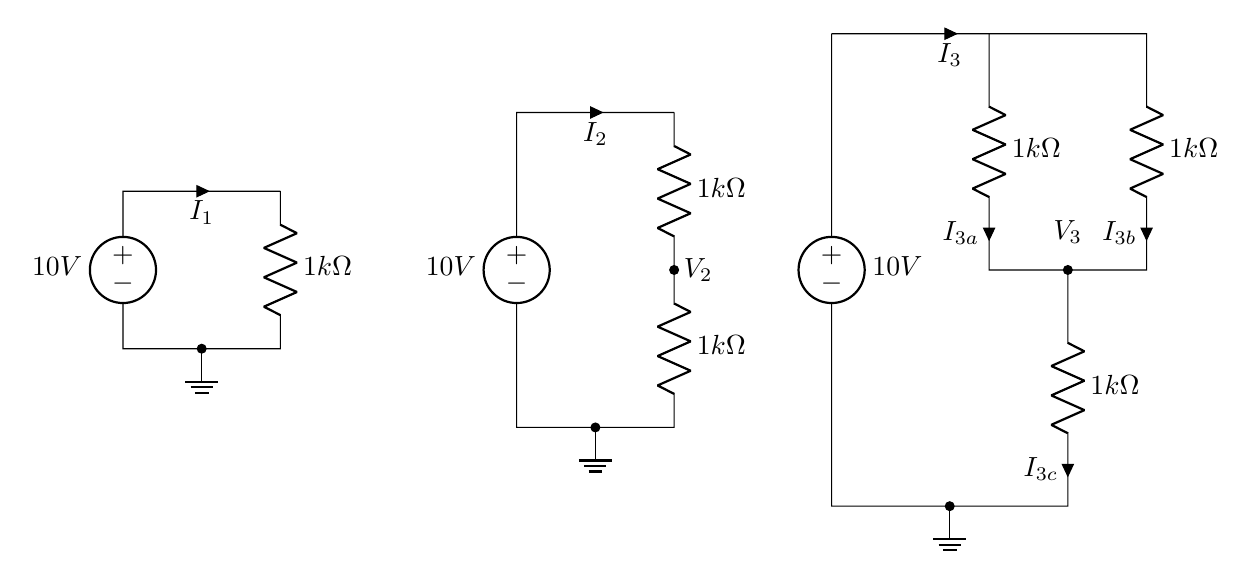
\begin{tikzpicture}
  			\draw
  			(2,-1)  to[R, l=$1 k\Omega$] ++ (0,-2)
  			to[short] ++ (-1,0) node[ground]{} ++ (-1,0);
  			\draw (1,-3) to[short, *-] ++ (-1,0)  to[V, l=$10V$, invert] ++ (0,2)
  			to[short, i_=$I_1$] ++ (+2,0);
  			
  			\draw
  			(7,0)  to[R, l=$1 k\Omega$, -*] ++ (0,-2)  node[anchor=west] {$V_2$}
  			to[R, l=$1 k\Omega$] ++ (0,-2)
  			to[short] ++ (-1,0) node[ground]{} ++ (-1,0);
  			\draw (6,-4) to[short, *-] ++ (-1,0)  to[V, l=$10V$, invert] ++ (0,4)
  			to[short, i_=$I_2$] ++ (+2,0);
  			
  			\draw
  			(11,1)  to[R, l=$1 k\Omega$,i_=$I_{3a}$] ++ (0,-3)
  			to[short] ++ (1,0);
  			\draw
  			(11,1) to[short] ++ (2,0)  to[R, l=$1 k\Omega$, i_=$I_{3b}$] ++ (0,-3)
  			to[short,-*] ++ (-1,0) to[R, l=$1 k\Omega$, i_=$I_{3c}$] ++ (0,-3)
  			to[short] ++ (-1.5,0) node[ground]{} ++ (-1,0);
  			\draw (9,1)  to[short,-] ++ (1,0) to[short,i_=$I_{3}$] ++ (1,0);
  			\draw (9,1) to[V, l=$10V$] ++ (0,-6)
  			to[short,-*] ++ (1.5,0);
  			\draw (12,-1.25) node[anchor=north] {$V_3$};
  		\end{tikzpicture}
  \caption{Resistive networks}
\end{figure}

\clearpage

\noindent\textbf{Label:} \texttt{fig:seriesparallel}\\[0.5em]
\begin{figure}[H]
  \centering
  \begin{circuitikz}[american]
  		\draw
  		(11,1)  to[R, l=$R1$] ++ (0,-3)
  		to[short] ++ (1,0);
  		\draw
  		(11,1) to[short] ++ (2,0)  to[R, l=$R2$] ++ (0,-3)
  		to[short,-*] ++ (-1,0) to[R, l=$R3$] ++ (0,-3)
  		to[short,-] ++ (-3,0);
  		\draw (9,1)  to[short,-] ++ (1,0) to[short] ++ (1,0);
  		\draw (9,1) to[V, l=$5V$] ++ (0,-3)
  		to[short,-] ++ (-0.5,0) node[ground]{} ++ (1,0);
  		\draw (9,-2) to[V, l=$5V$] ++ (0,-3);
  		\draw (12,-1.25) node[anchor=north] {$V_3$};
  	\end{circuitikz}
  \caption{Series-parallel resistive network with two stacked 5 V supplies. R1 and R2 are in parallel; their combination is in series with R3. Node V3 marks the junction between the parallel and series sections.}
\end{figure}

\clearpage

\noindent\textbf{Label:} \texttt{fig:acpec}\\[0.5em]
\begin{figure}[H]
  \centering
  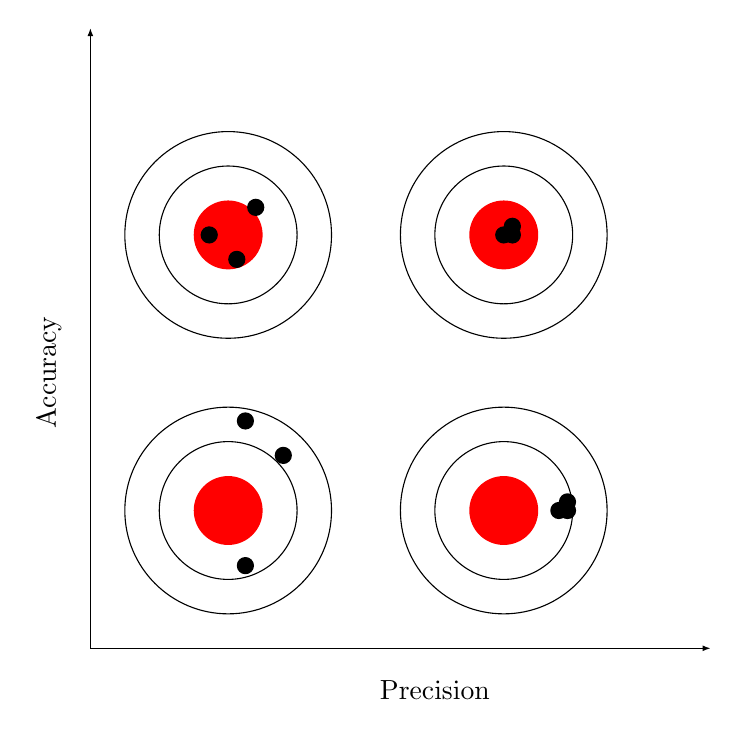
\begin{tikzpicture}[scale=3.5]
  		\def\radiusOne{1/8}
  		\def\radiusTwo{2/8}
  		\def\radiusThree{3/8}
  		\def\radiusFour{4/8}
  		\fill[red] (0,0) circle (\radiusOne);
  		\draw (0,0) circle (\radiusTwo);
  		\draw (0,0) circle (\radiusThree);
  		\fill[black] (+0.2,+0.2) circle (1/32);
  		\fill[black] (0+0.125/2,-0.2) circle (1/32);
  		\fill[black] (0+0.125/2,0+0.125+0.2) circle (1/32);
  		\fill[red] (1,1) circle (\radiusOne);
  		\draw (1,1) circle (\radiusTwo);
  		\draw (1,1) circle (\radiusThree);
  		\fill[black] (1,1) circle (1/32);
  		\fill[black] (1+0.125/4,1) circle (1/32);
  		\fill[black] (1+0.125/4,1+0.125/4) circle (1/32);
  		\fill[red] (1,0) circle (\radiusOne);
  		\draw (1,0) circle (\radiusTwo);
  		\draw (1,0) circle (\radiusThree);
  		\fill[black] (1+0.2,0) circle (1/32);
  		\fill[black] (1+0.2+0.125/4,0) circle (1/32);
  		\fill[black] (1+0.2+0.125/4,0+0.125/4) circle (1/32);
  		\fill[red] (0,1) circle (\radiusOne);
  		\draw (0,1) circle (\radiusTwo);
  		\draw (0,1) circle (\radiusThree);
  		\fill[black] (0.1,1.1) circle (1/32);
  		\fill[black] (-0.1+0.125/4,1) circle (1/32);
  		\fill[black] (0+0.125/4,1-0.12+0.125/4) circle (1/32);
  		\draw[-{Latex[length=1mm]}] (-1/2,-1/2) -- (1.75,-1/2);
  		\draw[-{Latex[length=1mm]}] (-1/2,-1/2) -- (-1/2,1.75);
  		\node[rotate=90] at (-3/4+0.1, 0.5) {Accuracy};
  		\node at (3/4, -3/4+0.1) {Precision};
  	\end{tikzpicture}
  \caption{Measurement analogy: High precision refers to how consistently repeated measurements cluster together, regardless of whether they are near the true value. Resolution represents the smallest increment a measuring instrument can detect. The top right bullseye demonstrates both excellent precision and accuracy. The top left shows good accuracy but poor precision. When making real-world measurements, you do not know the true value beforehand; you must rely on your instrument's precision and accuracy capabilities to estimate it.}
\end{figure}

\clearpage

\noindent\textbf{Label:} \texttt{fig:Lab3Fig1211}\\[0.5em]
\begin{figure}[H]
  \centering
  \begin{circuitikz}[american]
  			\draw (7,0) node[anchor=west] {$V_a$}
  			to[R, l=$820\,\Omega$, -*] ++ (0,-2)
  			node[anchor=west] {$V_b$}
  			to[R, l=$1.2\,k\Omega$] ++ (0,-2)
  			node[anchor=west] {$V_c$}
  			to[short, *-] ++ (-1,0);
  			\draw (6,-4) to[short, -] ++ (-1,0)
  			to[V, l=$5V$, invert] ++ (0,2)
  			to[short, -] ++ (-1,0) node[ground]{};
  			\draw (7,0) to[short, -] ++ (-2,0)
  			to[V, l=$5V$] ++ (0,-2);
  			\node[anchor=east] at (6.8,-2.5) {\textrm{R$_1$}};
  			\node[anchor=east] at (6.8,-0.5) {\textrm{R$_2$}};
  		\end{circuitikz}
  \caption{Resistive network \#1}
\end{figure}

\clearpage

\noindent\textbf{Label:} \texttt{fig:resistivenet2}\\[0.5em]
\begin{figure}[H]
  \centering
  \begin{circuitikz}
  			\draw
  			(11,1) to[R, l=$820\,\Omega$,i_=$I_{3a}$] ++ (0,-3)
  			to[short] ++ (1,0);
  			\draw
  			(11,1) to[short] ++ (2,0) node[anchor=west] {$V_a$}
  			to[R, l=$1\,k\Omega$, i_=$I_{3b}$] ++ (0,-3)
  			to[short,-*] ++ (-1,0)
  			to[R, l=$1.2\,k\Omega$, i_=$I_{3c}$] ++ (0,-3)
  			node[anchor=west] {$V_c$}
  			to[short] ++ (-1.5,0);
  			\draw (9,1) to[short,-] ++ (1,0) to[short,i_=$I_{3}$] ++ (1,0);
  			\draw (9,1) to[V, l=$10V$] ++ (0,-6)
  			to[short,-] ++ (1.5,0);
  			\draw (12,-1.25) node[anchor=north] {$V_b$};
  			\node[anchor=east] at (10.83,-0.25) {\textrm{R$_2$}};
  			\node[anchor=east] at (12.83,-0.25) {\textrm{R$_3$}};
  			\node[anchor=east] at (11.83,-3.25) {\textrm{R$_1$}};
  		\end{circuitikz}
  \caption{Resistive network \#2. Note that grounds are not explicitly shown in this circuit. You need to decide where to place them. Hint: See Figure~\ref{fig:Lab3Fig1211}.}
\end{figure}

\clearpage

\noindent\textbf{Label:} \texttt{fig:labConnnection1}\\[0.5em]
\begin{figure}[H]
  \centering
  \begin{circuitikz}[american]
  				\ctikzset{bipoles/oscope/waveform=none}
  				\draw (0,0) to[short, -o] ++(1,0)
  				to[short] ++ (1,0)
  				to[vsourcesin] ++(-0,-3)
  				node[ground]{};
  				\draw (0,0) to[oscope] ++(0,-3)
  				node[ground]{};
  				\node[anchor=south] at (-0.6,-1) {\textrm{Ch1+}};
  				\node[anchor=south] at (-0.6,-1-1.6) {\textrm{Ch1-}};
  				\node[anchor=south] at (2.5,-1) {\textrm{W1}};
  				\node[anchor=south] at (2.6,-3.4) {\textrm{\tiny{internal}}};
  				\draw (6,0) to[short, -o] ++(1,0)
  				to[short] ++ (1,0)
  				to[vsourcesin] ++(-0,-3)
  				node[ground]{};
  				\draw (6,0) to[oscope] ++(0,-3)
  				node[ground]{};
  				\node[anchor=south] at (-0.6+6,-1) {\textrm{Ch2+}};
  				\node[anchor=south] at (-0.6+6,-1-1.6) {\textrm{Ch2-}};
  				\node[anchor=south] at (2.5+6,-1) {\textrm{W2}};
  				\node[anchor=south] at (2.6+6,-3.4) {\textrm{\tiny{internal}}};
  			\end{circuitikz}
  \caption{M2K signal generation channels and oscilloscope channels. This configuration creates single-ended measurements of the generated signals.}
\end{figure}

\end{document}
